\section{Architecture}
In this work, the most important decision of the architecture was the choice of using Vulkan for the graphics API. Using Vulkan has been a learning process, and the architecture chosen reflects it.

In order to have our Vulkan code respond to changes in the control window, some of the classes in our architecture are exposed to GDScript via GDNative. GDNative requires the developer to register each method and property that will be made available for engine scripts to call, which allows our application to provide a minimal interface, keeping the implementation encapsulated, separated from the GUI in the control window.

Since GDNative loads a precompiled dynamic library, it is required for the developer to provide the library for the platforms to which the project is to be deployed. The development of our application was completely done in Linux, and thus it is the only platform the library has been compiled into, but our code does not rely on any platform-dependent libraries, so compiling to Windows or MacOS should be straightforward.

The architecture of Shader Tutor is depicted in Figure \ref{fig:architecture}. The purpose of each module is described in the following sections.

\begin{figure}[h]
    \caption{Shader Tutor architecture}
    \begin{center}
        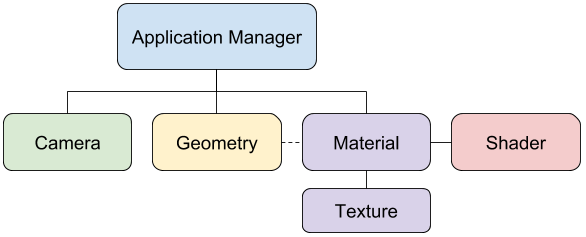
\includegraphics[width = 15cm]{figs/ShaderTutorArchitecture.png}
    \end{center}
    \legend{Source: the author}
    \label{fig:architecture}
\end{figure}

\subsection{Vulkan Application Module}
Vulkan is a low-level API and, as such, requires developers to setup a large amount of objects and configurations before displaying anything on screen. This module is responsible for creating these objects required for rendering.

\subsubsection{Vulkan Instance}
There is no global state in Vulkan and all per-application state is stored in a VkInstance object. Creating a VkInstance object initializes the Vulkan library and allows the application to pass information about itself to the implementation \cite{vulkan_docs}. Applications can even define and manage multiple instances if they so desire.

In order to initialize a Vulkan instance object, we first need to create a VkApplicationInfo structure object, which will describe our application for the driver. This structure hold the name and version of the application, and also the name and version of the engine used. This data is technically optional, but it may provide some useful information to the driver to optimize for our specific application, for example because it uses a well-known graphics engine with certain special behavior \cite{vulkan_tutorial}. Unlike the VkApplicationInfo, the VkInstanceCreateInfo structure object is not optional. It describes the instance extensions and debug layers we want to enable in our application. To make sure our application can be executed, we can check the available extensions with the function vkEnumerateInstanceExtensionProperties to compare against our required extensions. In our application, we are using GLFW for window management, which provides the glfwGetRequiredInstanceExtensions function \cite{glfw_vulkan} to query the required functions for surface creation on any platform supported by the library.

During the Vulkan instance object creation we can also specify validation layers to be enabled. Available validation layers can be queried with the vkEnumerateInstanceLayerProperties function. The Vulkan SDK provides a standard validation layer, "VK\_LAYER\_LUNARG\_standard\_validation", which implicitly enables a range of useful diagnostic layers. In order to receive the debug messages from the validation layers, however, the application must also enable the "VK\_EXT\_debug\_report" extension, which will allow the developer to setup a callback function that will be called whenever a debug message is issued by the validation layers. To setup the debug callback function, the developer has to get a pointer to the vkCreateDebugReportCallbackEXT, which is an extension function and therefore not included in the base API, using the vkGetInstanceProcAddr function.

\subsubsection{Physical Device}
The function vkEnumeratePhysicalDevices returns a list of available Vulkan devices installed in the system. Basic device properties like the name, type and supported Vulkan version can be queried using vkGetPhysicalDeviceProperties. The support for optional features like texture compression, 64 bit floats and multi viewport rendering can be queried using vkGetPhysicalDeviceFeatures. Device features must be enabled before they are used by the application.

Almost every operation in Vulkan, from drawing to uploading textures, requires commands to be submitted to a queue. A queue belongs to a \emph{queue family}, and each queue family supports certain types of commands. For a rendering application like ours, we need a queue able to render graphics, and another queue for presentation (displaying images in the window). These queues could be the same, if the physical device presents a single queue with both graphics and presentation capabilities. To query queue families, there is a vkGetPhysicalDeviceQueueFamilyProperties function.

With a list of the available devices, their features and queue families, we can select a VkPhysicalDevice and create a logical device to interface with it.

\subsubsection{Device}
The logical device creation process is similar to the instance creation process and describes the features we want to use in our application. We also need to specify which queues to create from the queue families that are available. 

The function vkCreateDevice takes the physical device we selected and a VkDeviceCreateInfo object as arguments. The latter describes which physical device features we want to enable from our selected physical device. We must also specify the queues we want to create, indicating the queue family index and amount of queues we want to create from each family. After the device is created, the application can call the vkGetDeviceQueue function to get the VkQueue objects to which commands will be passed into.

\subsubsection{Window Surface}



\subsection{Shader Module}
A Shader object represents one stage of the programmable pipeline stages. This module has a type indication, either vertex or fragment, and is capable of loading GLSL source files and compiling them into SPIR-V binary using the ShaderC library, developed by Google. The compiled code is then enclosed by a 'VkShaderModule' object which will be used in a material's graphics pipeline.

The type of the shader is inferred when a GLSL shader file is loaded based on the extension of the shader file, '.vert' for a vertex shader and '.frag' for a fragment shader.

This module also provides ways to check the compilation status and get any compilation error messages.


\subsection{Material Module}
A Material is a combination of a vertex and a fragment shader, plus the values of the uniform variables defined in those shaders. It is responsible for the creation of the Vulkan graphics pipeline object, based on the shaders loaded into it and other configuration values.

\subsubsection{Shader Parsing}
The shaders added to the material will have their SPIR-V code parsed by the \emph{SPIRV Cross} library. Our application will use this data to load the appropriate vertex attributes, uniform objects and sampler objects used by the shaders.

Shaders define which vertex attributes will be used as input, and uniform variables can serve as parameters for the material. All vertex attributes must be recognized by our application, following the defined names and types defined in table \ref{tab:vertex_attributes}. The user can also query the application for certain uniform variables, following the names and types defined in Table \ref{tab:uniform_variables}.

\begin{table}[h]
    \centering
    \caption{Recognized vertex attributes}
    \begin{tabular}{|c|c|p{6cm}|}
    \hline
        \textit{Type} & \textit{Name} & \textit{Description} \\
        \hline \hline
        vec3 or vec4 & \texttt{position} & Vertex position \\
        vec3 or vec4 & \texttt{normal} & Normal vector of the surface \\
        vec3 or vec4 & \texttt{tangent} & Tangent vector to the surface \\
        vec2 & \texttt{uv} & Texture coordinate \\
        \hline
    \end{tabular}
    \label{tab:vertex_attributes}
\end{table}

If the \texttt{position} attribute is a vec4, the fourth component will be set to one; If the \texttt{normal} is a vec4, the fourth component will be set to zero; If the \texttt{tangent} is a vec4, the fourth component will be either set do 1 or -1, indicating the direction pointed by the binormal vector, used in normal mapping.

\begin{table}[h]
    \centering
    \caption{Recognized uniform variables}
    \begin{tabular}{|c|c|p{6cm}|}
        \hline
        \textit{Type} & \textit{Name} & \textit{Description} \\
        \hline
        \hline
        mat4 & \texttt{model} & Model matrix \\
        mat4 & \texttt{view} & View matrix \\
        mat4 & \texttt{projection} & Projection matrix \\
        mat4 & \texttt{modelView} & Model-View matrix \\
        mat4 & \texttt{modelViewProjection} & Model-View-Projection matrix \\
        mat4 & \texttt{modelInverse} & Model matrix inverse \\
        mat4 & \texttt{viewInverse} & View matrix inverse \\
        mat4 & \texttt{projectionInverse} & Projection matrix inverse \\
        mat4 & \texttt{modelViewInverse} & Model-View matrix inverse \\
        mat4 & \texttt{modelViewProjectionInverse} & Model-View-Projection matrix inverse \\
        mat3 & \texttt{normalMatrix} & Matrix to transform the normal vectors of the object; Corresponds to the inverse transposed 3x3 model-view submatrix \\
        \hline
    \end{tabular}
    \label{tab:uniform_variables}
\end{table}

Note that the normal matrix is a 3x3 matrix, unlike the other ones. This is because the correct matrix to transform the normal vector is the transpose of the inverse of the 3x3 submatrix from the model view matrix \cite{normal_matrix}.

The shader code can also define arbitrary uniform variables, which will be initialized to a default value and exposed in the control window so the user can change the values manually. Numeric values are initialized to 1 to avoid division by zero. Image samplers defined in code will be initialized to a white texture.

\subsubsection{Descriptor set layout and descriptor pool}
After the shaders are parsed, the Material module will create the descriptor set layout object ('VkDescriptorSetLayout') and descriptor pool. In our case, every uniform buffer object and image sampler is available in all graphics stages (vertex and fragment). For this reason, the shaders must declare the binding of each uniform buffer object and image sampler used in GLSL code, and the binding numbers cannot be reused. This is done in GLSL by using the layout qualifier in the declaration of the uniforms.

For our application, the size of the descriptor pool translates into how many different objects can have the same material applied at a given time.


\subsection{Geometry Module}
The geometry module represents an object in the scene. It holds all the vertices attributes (vertex position, normal, tangent, texture coordinates and indices, if available); a transformation, which defines the rotation, scale and translation applied to the object; and a reference to a material object which will be used to render the geometry in the scene.

\subsubsection{Vertex, Index and Uniform Buffers}
When an object is added to the scene, it must be filled with vertex data and then a material has to be assigned to the material. Then, the object will get a list of the required vertex attributes from the material, and create the vertex buffer accordingly. If the vertex attributes include index data, the index buffer is created, too. Then, the uniform buffers are created, based on the uniform buffer objects in the material assigned.

\subsubsection{Descriptor Sets}
For the uniform buffer to be passed to the shaders, we need to allocate a descriptor set from the pool defined in the material assigned to this geometry. We need to do this because the descriptor layout in the material is just a description of what types of descriptors can be bound, but no uniform buffer has been referenced yet. The descriptor set specifies a buffer to be bound in the uniform buffer descriptor.

\subsubsection{Recording Drawing Commands}
Since all drawing operations are recorded in advance in Vulkan, this module also provides a method for recording the drawing commands in a command buffer previously initialized.

\subsubsection{Updating Uniform Buffers}
The function to update uniform buffers is called by the Vulkan application module, and expects a structures containing certain uniform values that are not dependent on the object, such as the camera's view and projection matrices. The other matrices are calculated and loaded into the appropriate buffers.

The material can define arbitrary uniform variables, and those must be updated as well. The material holds an array of dictionaries that describe each of the user-defined variables, their types, sizes, bindings, offsets and values. With this information, our application is able to load the variable value into the correct buffer in the correct offset.


\subsection{Texture Module}
The texture module handles the passage of image data for the shaders. This means creating an image, allocating device memory for the image, creating the image view and the sampler.

Image files are loaded by Godot, the engine used to create the user interface, and their data is passed to the texture module. Our application then has to pass this data into the device memory bound to the image. However, there is no way to write directly to the image memory, which forces us to use a \textit{staging buffer}. The staging buffer can be mapped to CPU memory and accessed by our application. In order to transfer this data to the image, the image must have its layout transitioned to optimal for transfer destination. This is done using a single time command buffer, which is allocated, recorded, executed and freed, sequentially. Single time command buffers are managed by the Vulkan application module. Once the image is ready to receive a data transfer and the staging buffer is loaded, we can use another single time command buffer to copy the buffer contents into the image. After this transfer is complete, the image must be transitioned again to a layout optimal for shader read only. Then, the staging buffer can be destroyed, and the device memory can be freed.


\subsection{Camera Module}
The camera module represents a virtual camera. It has a position, target and up vectors for reference and an angle for the field of view of the projection. This module provides the view and projection matrices used to transform the objects in the shaders. It also presents methods for moving and turning, used by the Vulkan application module.

